\documentclass[portrait]{sciposter}

\usepackage{graphicx}
\usepackage{amsmath}
\usepackage{multicol}


\title{Modeling the Dynamics of Vector-Host Interactions in Avian Communities for Eastern Equine Encephalitis Virus}

\author{\textit{Timothy Muller}\footnotemark[1]$^*$
and Goudarz Molaei\footnotemark[2], Michael C. Thomas\footnotemark[2], John J. Shepard\footnotemark[2], Philip M. Armstrong\footnotemark[2], Theodore G. Andreadis\footnotemark[2], Jan Medlock\footnotemark[3]}

\institute{
  \footnotemark[1]$^*$ 
  Graduate Program in Comparative Health Sciences, 
  Division of Health Sciences, Oregon State University
  Presenting Author
  \texttt{mullert@onid.orst.edu}
  \\
  \footnotemark[2]
  Center for Vector Biology and Zoonotic Diseases,
  The Connecticut Agricultural Experiment Station,
  New Haven, CT
  \\
  \footnotemark[3]
  Department of Biomedical Sciences,
  Oregon State University,
  \texttt{jan.medlock@oregonstate.edu}}

%\renewcommand{\thefootnote}{\fnsymbol{footnote}}


\rightlogo{graphics/Vertical-spot}
\noleftlogo


\conference{ESA 2017, 6-11 August 2017}


\newcommand{\md}{\mathrm{d}}
\newcommand{\me}{\mathrm{e}}
\newcommand{\mT}{\mathrm{T}}
\renewcommand{\vec}[1]{\mathbf{#1}}
\newcommand{\mat}[1]{\mathbf{#1}}
\DeclareMathOperator{\Prob}{Prob}
\DeclareMathOperator{\E}{E}
\DeclareMathOperator{\Bernoulli}{Bernoulli}
\DeclareMathOperator{\Multinomial}{Multinomial}
\DeclareMathOperator{\Poisson}{Poisson}


\renewcommand{\emph}[1]{\textcolor{red}{#1}}
\newcommand{\comment}[1]{\textcolor{blue}{#1}}


\begin{document}


\maketitle


\begin{multicols}{2}

  \section*{Introduction}
  \subsection*{Eastern Equine Encephalitis (EEE)}
  \begin{itemize}
\item EEE virus (Togaviridae, Alphavirus) is a highly pathogenic mosquito-borne zoonosis that is responsible for outbreaks of severe disease in humans and equines, resulting in high mortality or severe neurological impairment in most survivors.
\item In the past, outbreaks occurred intermittently with no apparent pattern; however, during the last decade we have witnessed annual reoccurrence of virus activity with human and equine cases
\end{itemize} 
    \subsection*{Vectors and Hosts}
\begin{itemize}
\item In the northeastern United States, EEE is maintained in an enzootic cycle involving the ornithophilic mosquito, \textit{Culiseta melanura} and a variety of passerine birds in freshwater swamp habitats. \\
\item It is believed that the various passerine bird hosts allows the disease to overwinter and survive despite a relative lack of mosquito presence
\end{itemize}

\section*{Data Collection}
\begin{itemize}
\item Over a period of several months, the Connecticut Agricultural Experiment Station (CAES) both collected samples of \textit{Culiseta melanura} and tracked the appearance of various bird species in set locations
\begin{center}
\includegraphics[width=.25\linewidth]{figs/EEESitefig}
\end{center}
\item 1127 blood meals were successfully collected and identified to species level
\item Greater than 99 percent were from 65 avian hosts in 27 families and 11 orders
\item Examination of the blood meals leads us to emphasize our analysis on 8  bird species
\end{itemize}

\section*{Parameters and Assumptions}
\subsection*{Feeding Index $\alpha$}
The feeding index $\alpha_i$ assesses the proportion of blood meals from a particular host species i in relation to the proportional abundance of that species in the host community.  Hence a feeding index of 1 indicates opportunistic feeding habits, while a feeding index greater than 1 indicates preferential feeding. \\
\begin{center}
\huge $\alpha_i= \frac{\frac{f_i}{\sum\limits_{j=1}^nf_j}}{\frac{N_i}{\sum\limits_{j=1}^nN_j}}$ 
\end{center}
Where $f_i$ is the number of blood meals obtained from a specific bird

\subsection*{Fixed Parameters}
Due to limited experimental data on the subject, the following were assumed to be fixed for the purposes of the model:
\begin{itemize}
\item Bird recruitment rate, $\textit{b}$ and bird death rate $\textit{d}$ 
\item Recovery rate $\gamma$ is assumed to be constant amongst all bird species
\item Mosquito death rate $d_v$ and vector biting rate \textit{v} 
\end{itemize}
Furthermore studies suggest that infection of a susceptible vector is guaranteed if they feed from of a viremic host, and thus the host-vector transmission rate $\beta_2$ is also fixed

\subsection*{Transmission Rates $\beta_i$}
\begin{itemize}
\item Studies suggest that vector-to-host transmission is guaranteed when an infectious vector feeds
from a host, and thus the vector-to-host transmission rate was set to 1. 
\item Limited data exists regarding the value of the host-to-vector transmission rate among the various host species. In
order to focus the analysis on the effect of variable biting rates on the model's output, the host-to-vector
transmission rate is assumed to be constant across all of the host species
\item The all-species host-to-vector transmission rate was determined by fitting the model proportion of birds that
became infected over the model period to the observed proportion of seropositives amongst the
various bird species from a previous study. 
\end{itemize}

\columnbreak
 
 \section*{Mathematical Model}
We choose to focus on 6 preferential host species, and a seventh consisting of all other birds.  This leaves us with a system of 23 differential equations (with i=1,2,...,9). \\
\begin{align*}
\frac{dS_i}{dt} &= \textit{b}N_i - \lambda_bS_i - \textit{d}S_i&  
\lambda_b &= \frac{\beta_1vI_v\sum\alpha_i}{\sum\alpha_iN_i} \\
\frac{dI_i}{dt} &=  \lambda_bS_i -  \gamma_bI_i-d_{EEE}I_i - \textit{d}I_i \\
\frac{dR_i}{dt} &= \gamma_bI_i - \textit{d}R_i&
\lambda_v &= \frac{\beta_2v\sum\alpha_II_i}{\sum\alpha_iN_i} \\
\frac{dI_v}{dt} &= \lambda_vS_v - d_vI_v \\
\frac{dS_v}{dt} &= r(t)N_v - d_vI_v&
\end{align*}

\section*{Interpolation Splines}
\begin{itemize}
\item Utilizing Markov chain Monte Carlo methods, 1000 samples were selected for both the counts and blood meals.
\item From each of these samples, the feeding indices for each of the selected bird species were calculated
\item We have reported the median and 95\% confidences intervals for the calculated proportion infected for each host species. 
\end{itemize}

\section*{Results}
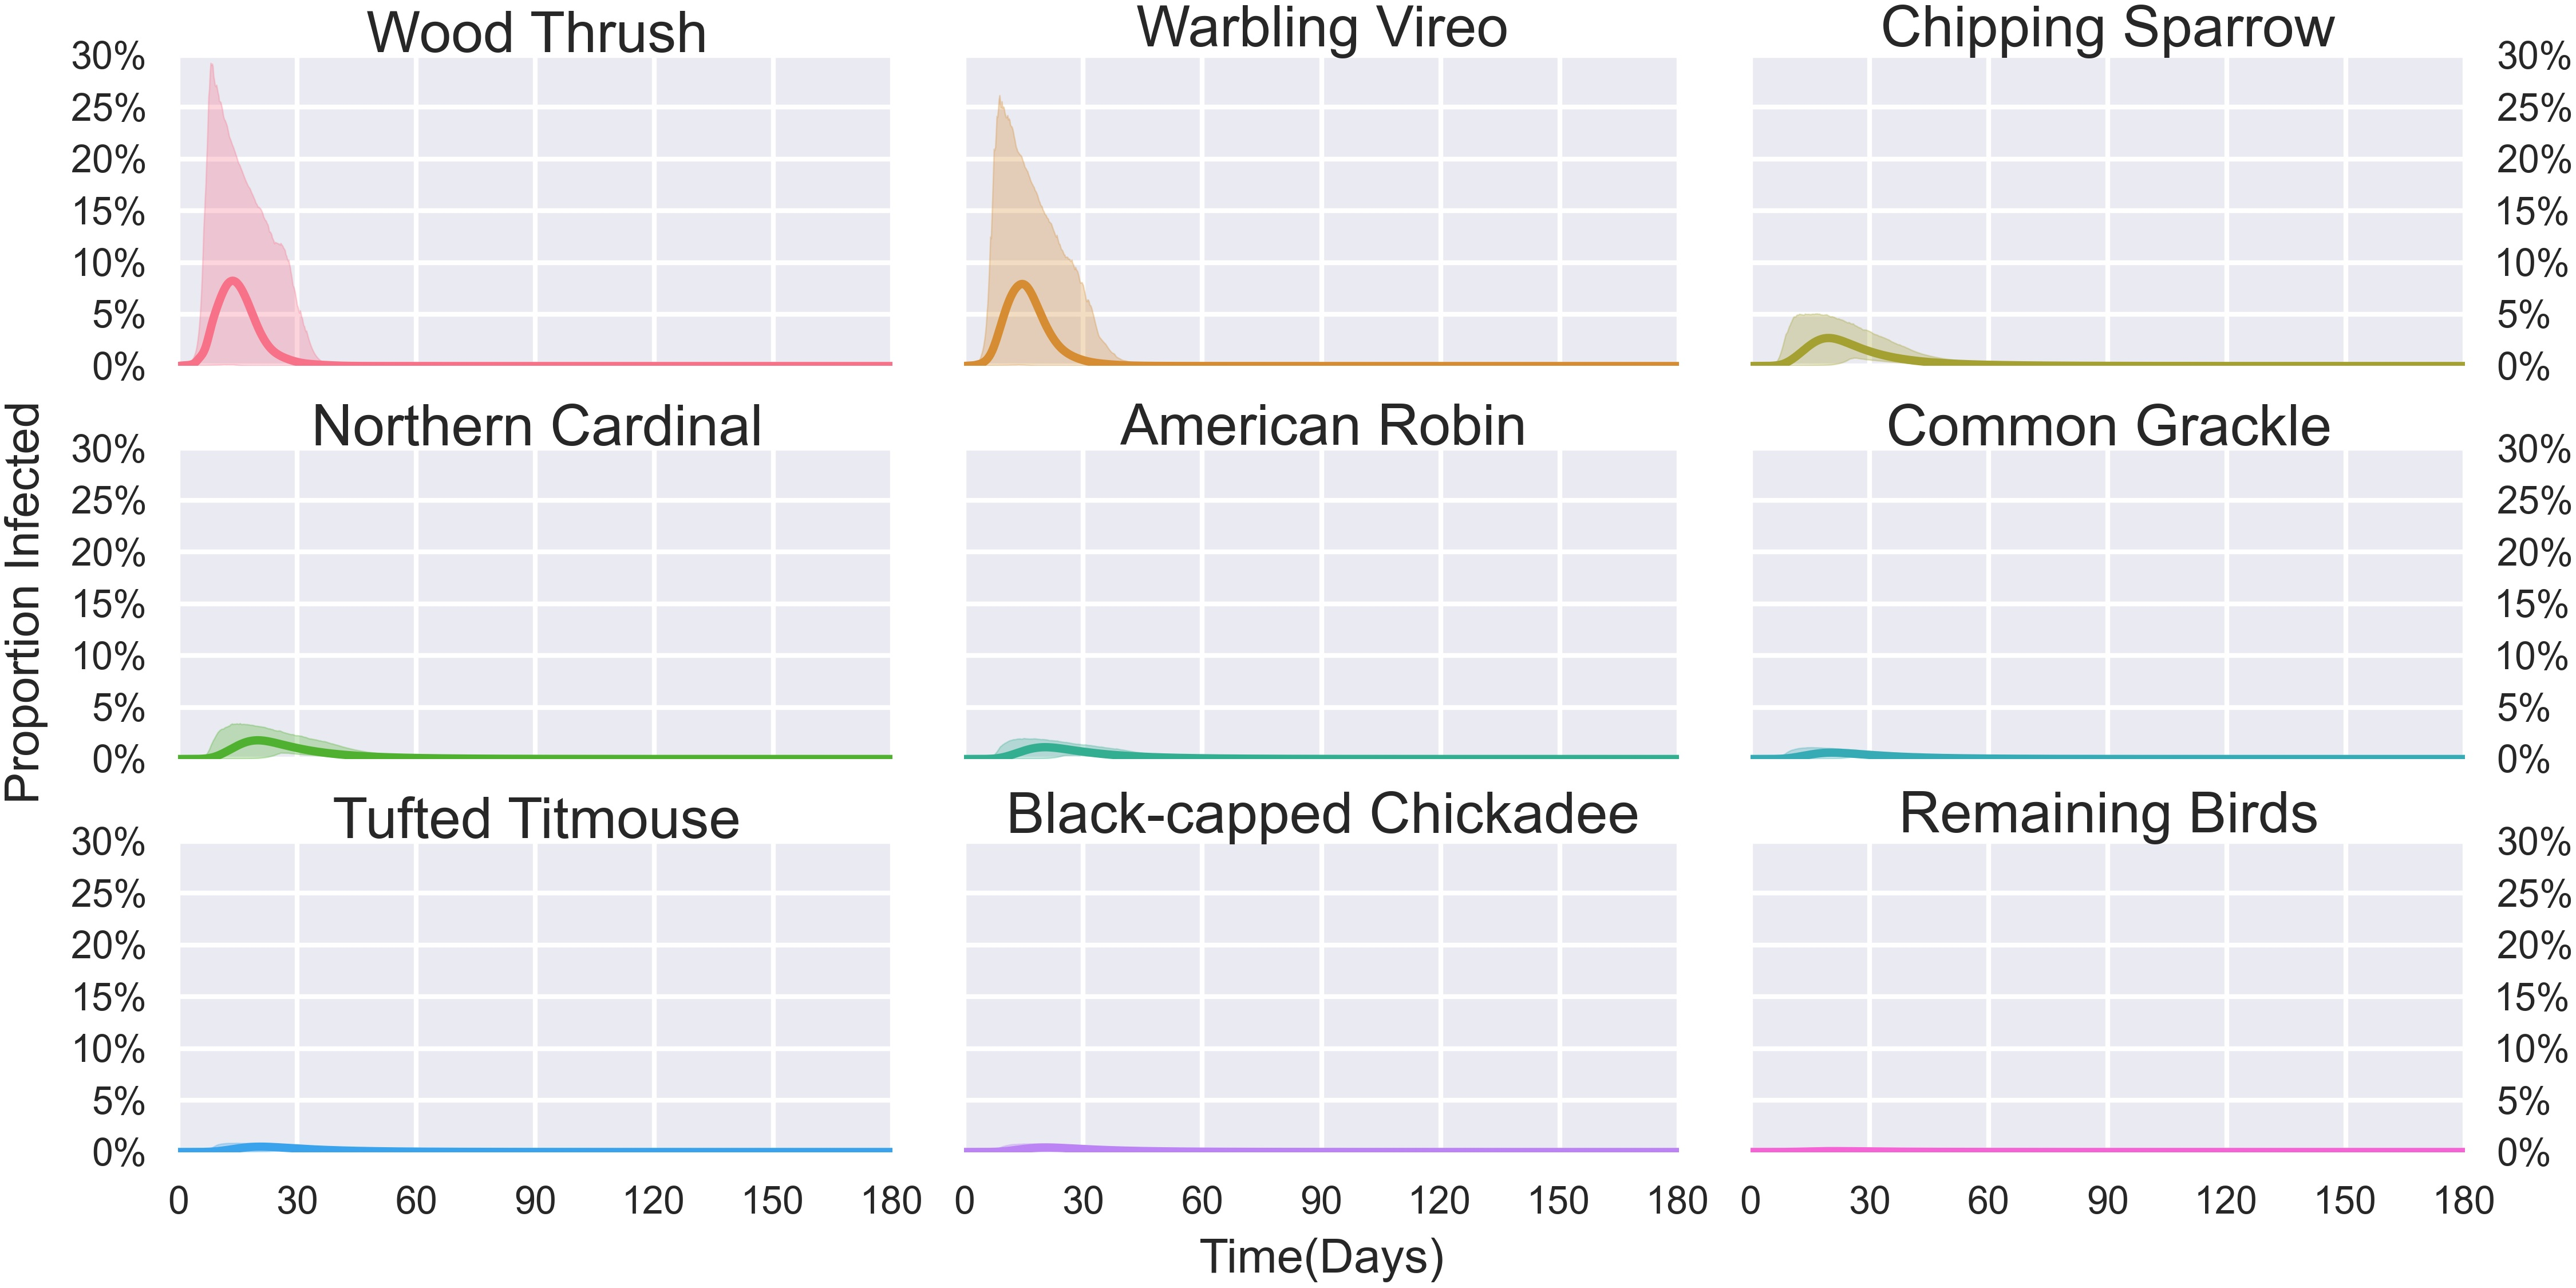
\includegraphics[width=\linewidth]{Results}

\section*{Conclusions and Future Work}
\subsection*{Conclusions}.

\subsection*{Future Questions}
\begin{itemize}

\subsection*{Funding}
Funded in part by NIH U01 GM070694

\end{multicols}


\end{document}
